% !TeX root = ../notes.tex 

\chapter{Quantitative approaches to reaction mechanisms}

\begin{notebox} 
    \keypoint{What do you need to learn from this chapter?}
    This chapter examines how quantitative experiments can be used to distinguish between competing reaction mechanisms. 
    You should understand how kinetic analysis, linear free-energy relationships, and other quantitative structure–reactivity relationships provide complementary mechanistic information. 
\end{notebox} 

\section{From observations to mechanism}

Reaction mechanisms are models inferred from experimental observations.
Different experiments probe different aspects of a reacting system, and a mechanistic proposal should account for the combined evidence rather than a single result.

A useful mechanistic experiment perturbs a chemical system in a way that allows competing explanations to be distinguished.
Concentration, molecular structure, and catalyst composition can be varied to probe kinetic behaviour, structure--reactivity relationships, and catalyst speciation.

\solution{8.5cm}{%
  \centering

  \resizebox{0.65\linewidth}{!}{%
    \begin{tikzpicture}[
        transform shape,
        input/.style={
          draw=darkBlue,
          fill=paleBlue,
          line width=2.0pt,
          minimum width=7.2cm,
          minimum height=1.05cm,
          align=center,
          font=\sffamily
        },
        process/.style={
          draw=darkRed,
          fill=paleRed,
          line width=2.0pt,
          minimum width=7.2cm,
          minimum height=1.05cm,
          align=center,
          font=\sffamily
        },
        result/.style={
          draw=darkGreen,
          fill=paleGreen,
          line width=2.0pt,
          minimum width=7.2cm,
          minimum height=1.05cm,
          align=center,
          font=\sffamily
        },
        arrow/.style={
          ->,
          >=Stealth,
          draw=darkGrey,
          line width=2.5pt
        },
        feedback/.style={
          ->,
          >=Stealth,
          draw=darkGrey,
          dashed,
          line width=2.0pt
        },
        feedbacklabel/.style={
          font=\small\sffamily,
          text=darkGrey,
          align=center,
          fill=paleYellow,
          inner sep=2pt
        }
      ]

      \path[use as bounding box] (-5.2,-0.3) rectangle (4.1,9.2);

      \node[input] (perturb) at (0,8.3)
      {
        \textbf{Perturb}\\[-1pt]
        {\small concentration, structure, composition}
      };

      \node[input] (measure) at (0,6.0)
      {
        \textbf{Measure}\\[-1pt]
        {\small rate, selectivity, products}
      };

      \node[process] (compare) at (0,3.7)
      {
        \textbf{Compare with model}\\[-1pt]
        {\small expected relationship}
      };

      \node[result] (interpret) at (0,1.4)
      {
        \textbf{Interpret}\\[-1pt]
        {\small agreement or deviation}
      };

      \draw[arrow] (perturb) -- (measure);
      \draw[arrow] (measure) -- (compare);
      \draw[arrow] (compare) -- (interpret);

      \draw[feedback]
        (interpret.west)
        -- ++(-1.2,0)
        |- (perturb.west);

      \node[feedbacklabel,rotate=90] at (-4.85,4.85)
      {
        refine and repeat
      };

    \end{tikzpicture}%
  }
}

Agreement with a simple model supports its underlying assumptions.
Systematic deviation can instead reveal missing chemical behaviour and will be a recurring source of mechanistic information throughout this chapter.

\section{Kinetics and rate laws}

Kinetic experiments measure how reaction rate changes with composition and reaction progress.
The resulting rate law constrains a proposed mechanism but does not identify a unique sequence of elementary steps.
This section briefly reviews rate laws before focusing on reaction progress kinetic analysis and variable time normalisation analysis.

For a reaction involving substrates \textbf{A} and \textbf{B} and a catalyst, an empirical rate law can be written as

\solution{2.3cm}{%
  \begin{equation}
    r
    = -\frac{\mathrm{d}[\text{\textbf{A}}]}{\mathrm{d}t}
    = k_{\mathrm{obs}}
      [\text{\textbf{A}}]^{\alpha}
      [\text{\textbf{B}}]^{\beta}
      [\mathrm{cat}]^{\gamma}.
  \end{equation}
}

The exponents \(\alpha\), \(\beta\), and \(\gamma\) are experimental reaction orders.
They describe how the observed rate responds to concentration and are not necessarily equal to stoichiometric coefficients in the overall reaction.
For a catalytic reaction, an order can connect the catalyst resting state and substrate concentrations to the transition state controlling turnover.

The rate-determining step is often described as the elementary step with the greatest influence on the overall rate.
For a multistep catalytic reaction, the relevant activation barrier is measured from the populated resting state to the transition state that controls turnover.

\solution{7cm}{%
  \centering

  \resizebox{\linewidth}{!}{%
    \begin{tikzpicture}[
        transform shape,
        axis/.style={draw=darkGrey,line width=1.5pt,->,>=Stealth},
        profile/.style={draw=darkBlue,line width=2.6pt},
        barrier/.style={draw=darkRed,line width=1.8pt,<->,>=Stealth},
        guide/.style={draw=darkGrey,dashed,line width=1.0pt},
        label/.style={font=\small\sffamily,text=darkGrey,align=center}
      ]

      \path[use as bounding box] (0,-0.25) rectangle (17.3,5.8);

      % Axes
      \draw[axis] (1.15,0.2) -- (16.35,0.20);
      \draw[axis] (1.15,0.2) -- (1.15,5.25);
      \node[label,anchor=east] at (16.20,-0.3) {reaction coordinate};
      \node[label,rotate=90] at (0.52,4.15) {free energy, $G$};

      % Smooth catalytic energy profile
      \draw[profile]
        (2.1,1.60)
        .. controls (3.20,1.60) and (3.55,3.55) .. (4.65,3.55)
        .. controls (5.55,3.55) and (5.85,1.35) .. (7.65,1.35)
        .. controls (9.00,1.35) and (9.30,4.55) .. (10.55,4.55)
        .. controls (11.65,4.55) and (11.95,1.15) .. (14.75,1.15);

      % Minimal labels
      \node[label,anchor=south] at (2,1.9) {reactants};
      \node[label,anchor=north] at (7.65,1.23) {resting state};
      \node[label,anchor=south] at (14.75,1.28) {products};

      \node[label,text=darkRed,anchor=south] at (10.55,4.70)
        {turnover-controlling TS};

      % Effective turnover barrier, positioned in clear space
      \draw[guide] (7.65,1.35) -- (9.15,1.35);
      \draw[guide] (10.55,4.55) -- (9.15,4.55);
      \draw[barrier] (9.15,1.38) -- (9.15,4.52);
      \node[
        font=\small\sffamily,
        text=darkRed,
        anchor=east,
        align=right
      ] at (8.90,2.95)
        {$\Delta G^{\ddagger}_{\mathrm{turnover}}$};

    \end{tikzpicture}%
  }
}

Reaction order is commonly introduced through initial-rate measurements.
The slope of a plot of \(\ln r_0\) against \(\ln[\text{\textbf{A}}]\) gives the order in \textbf{A} when other concentrations are kept constant.
However, initial-rate analysis uses only a small part of each reaction profile and can miss behaviour that develops as substrates are consumed and products accumulate.
Reaction progress methods instead use concentration--time data across a larger fraction of the reaction.

\begin{warningbox}
  Linearisation can distort experimental error and make an assumed relationship appear more convincing than it is.
  A straight line does not establish that the proposed rate law or mechanism is correct.
\end{warningbox}

\solution{8.0cm}{%
  \begin{align}
    r_0 &= k'[\text{\textbf{A}}]^{\alpha}, \\
    \ln r_0 &= \alpha \ln[\text{\textbf{A}}] + \ln k'.
  \end{align}
  \\[1em]
  \centering

    \resizebox{\linewidth}{!}{%
      \begin{tikzpicture}[
          transform shape,
          axis/.style={draw=darkGrey,line width=1.5pt,->,>=Stealth},
          datum/.style={darkBlue,fill=darkBlue},
          fit/.style={draw=darkRed,line width=2.3pt},
          arrow/.style={->,>=Stealth,draw=darkGrey,line width=2.2pt},
          title/.style={font=\sffamily},
          label/.style={font=\small\sffamily,text=darkGrey,align=center}
        ]

        \path[use as bounding box] (0,-0.6) rectangle (17.3,5.2);

        % Raw power-law relationship
        \node[title] at (4.0,4.75) {Initial-rate data};
        \draw[axis] (1.0,0.7) -- (7.0,0.7);
        \draw[axis] (1.0,0.7) -- (1.0,4.3);
        \node[label] at (6.05,0.25) {$[\text{\textbf{A}}]_0$};
        \node[label,rotate=90] at (0.55,3.35) {$r_0$};

        \draw[fit]
          plot[domain=1.35:6.15,samples=80,variable=\x]
          (\x,{0.82 + 0.135*(\x - 1.15)^2});

        \foreach \x/\y in {
          1.45/0.83,
          2.10/0.94,
          2.80/1.19,
          3.50/1.57,
          4.20/2.08,
          4.90/2.72,
          5.60/3.49,
          6.10/4.13
        } {
          \fill[datum] (\x,\y) circle (3pt);
        }

        \draw[arrow] (7.55,2.45) -- (9.75,2.45);
        \node[label] at (8.65,2.88) {linearise};

        % Log--log relationship
        \node[title] at (13.25,4.75) {Linearised plot};
        \draw[axis] (10.25,0.7) -- (16.25,0.7);
        \draw[axis] (10.25,0.7) -- (10.25,4.3);
        \node[label] at (15.25,0.25) {$\ln[\text{\textbf{A}}]_0$};
        \node[label,rotate=90] at (9.80,3.35) {$\ln r_0$};

        \draw[fit] (10.70,1.00) -- (15.75,3.90);

        \foreach \x/\y in {
          10.85/1.08,
          11.55/1.43,
          12.25/1.82,
          12.95/2.23,
          13.65/2.62,
          14.35/3.05,
          15.05/3.43,
          15.65/3.82
        } {
          \fill[datum] (\x,\y) circle (3pt);
        }

      \end{tikzpicture}%
    }
}

\section{Visual kinetic analysis}

Initial-rate analysis uses only the beginning of each reaction profile, so most of the measured kinetic information is discarded.
It can miss behaviour that develops during the reaction, including product inhibition, catalyst deactivation, aggregation, or an induction period.
Reaction rate can change during a reaction for reasons other than depletion of the substrates.
Two common possibilities in catalytic reactions are \keypoint{catalyst deactivation} and \keypoint{product inhibition}.
In both cases, the reaction becomes slower than expected from substrate concentrations alone.
The useful mechanistic question is therefore how to compare reaction profiles in which the relevant concentrations are deliberately matched or changed.
This is the basis of \keypoint{reaction progress kinetic analysis}.\mcite{Blackmond2005}

\subsection{Reaction progress kinetic analysis}

Consider a catalytic reaction in which two molecules of compound \textbf{A} bind sequentially to the catalyst to form intermediate \textbf{I}$_2$.
Reaction with compound \textbf{B} then forms product \textbf{P} and regenerates the catalyst.
The catalyst may also undergo irreversible deactivation (Fig.~\ref{fig3-1:cycle}).

\begin{figure}[h!]
    \centering
    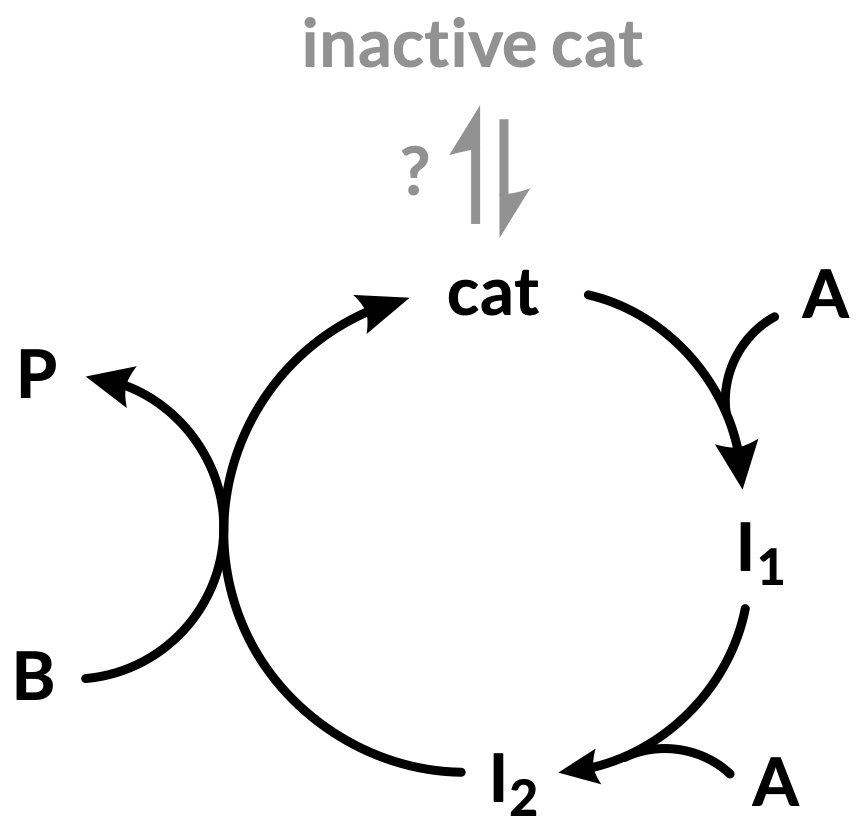
\includegraphics[width=5.4cm]{figures/CH3-cycle.png}
    \caption{A catalytic cycle with potential product inhibition.}
    \label{fig3-1:cycle}
\end{figure}

\keypoint{Reaction progress kinetic analysis (RPKA)} compares rates measured throughout complete reaction profiles.
Rate is plotted against a concentration that tracks reaction progress, so experiments are compared at matched compositions rather than matched times.

A \keypoint{same-excess experiment} is a new reaction started at substrate concentrations corresponding to a later point in the reference reaction.
The same-excess experiment therefore has the same substrate composition but a different reaction history: the catalyst is fresh and no product has yet accumulated unless it is added deliberately.

\solution{8.6cm}{%
  \centering

  \resizebox{\linewidth}{!}{%
    \begin{tikzpicture}[
        transform shape,
        axis/.style={draw=darkGrey,line width=1.5pt,->,>=Stealth},
        reference/.style={draw=paleRed,line width=3.2pt},
        same/.style={draw=paleBlue,line width=3.2pt},
        product/.style={draw=paleGreen,line width=3.2pt},
        datumref/.style={fill=darkRed,draw=darkRed,line width=0.5pt},
        datumsame/.style={fill=darkBlue,draw=darkBlue,line width=0.5pt},
        datumproduct/.style={fill=darkGreen,draw=darkGreen,line width=0.5pt},
        diagnostic/.style={draw=darkGrey,line width=1.7pt,->,>=Stealth},
        guide/.style={draw=darkGrey,dashed,line width=1.0pt},
        label/.style={font=\small\sffamily,text=darkGrey,align=center},
        title/.style={font=\sffamily,text=darkGrey,align=center}
      ]

      \path[use as bounding box] (0,-1.10) rectangle (17.3,7.75);

      % ==================================================
      % Product inhibition
      % ==================================================
      \node[title] at (4.15,7.28) {Product inhibition};
      \draw[axis] (0.8,1.0) -- (7.80,1.0);
      \draw[axis] (0.8,1.0) -- (0.8,6.70);
      \node[label,anchor=east] at (7.65,0.52) {$[\text{\textbf{A}}]$};
      \node[label,rotate=90] at (0.28,5.72) {rate};

      % Reference: r = 1.05 + 0.115([A]-1)^2
      \draw[reference]
        plot[domain=1.20:7.05,samples=100,variable=\x]
        (\x,{1.05 + 0.115*(\x - 1.00)^2});

      % Fresh same-excess: r = 1.55 + 0.155([A]-1)^2
      \draw[same]
        plot[domain=1.20:6.25,samples=100,variable=\x]
        (\x,{1.55 + 0.155*(\x - 1.00)^2});

      % Product-added reaction overlays the reference power law.
      \draw[product]
        plot[domain=1.20:7.05,samples=100,variable=\x]
        (\x,{1.05 + 0.115*(\x - 1.00)^2});

      % Filled circular data markers calculated from the same power laws.
      \foreach \x in {1.45,2.30,3.15,4.00,4.85,5.70,6.50,6.95} {
        \fill[datumref]
          (\x,{1.05 + 0.115*(\x - 1.00)^2}) circle (3.4pt);
      }
      \foreach \x in {1.55,2.40,3.25,4.10,4.95,5.70,6.15} {
        \fill[datumsame]
          (\x,{1.55 + 0.155*(\x - 1.00)^2}) circle (3.4pt);
      }
      \foreach \x in {1.65,2.50,3.35,4.20,5.05,5.90,6.60} {
        \fill[datumproduct]
          (\x,{1.05 + 0.115*(\x - 1.00)^2}) circle (3.4pt);
      }

      % Diagnostic arrow at one matched composition.
      \draw[guide] (4.45,1.0) -- (4.45,4.30);
      \draw[diagnostic]
        (4.45,{1.55 + 0.155*(4.45 - 1.00)^2})
        --
        (4.45,{1.05 + 0.115*(4.45 - 1.00)^2});
    %   \node[label,anchor=west] at (4.57,3.35)
    %     {$+\,\text{\textbf{P}}$};

      % Labels placed in unused upper-left area.
      \node[label,text=darkBlue,anchor=west] at (1.25,6.30)
        {same-excess with no product};
      \node[label,text=darkGreen,anchor=west] at (1.25,5.74)
        {$+\,\text{\textbf{P}}$: restores reference};

      % ==================================================
      % Catalyst deactivation
      % ==================================================
      \node[title] at (12.65,7.28) {Catalyst deactivation};
      \draw[axis] (9.30,1.0) -- (16.30,1.0);
      \draw[axis] (9.30,1.0) -- (9.30,6.70);
      \node[label,anchor=east] at (16.15,0.52) {$[\text{\textbf{A}}]$};
      \node[label,rotate=90] at (8.78,5.72) {rate};

      % Reference: lower power-law rate after catalyst ageing.
      \draw[reference]
        plot[domain=9.70:15.55,samples=100,variable=\x]
        (\x,{1.05 + 0.115*(\x - 9.50)^2});

      % Fresh same-excess: higher power-law rate.
      \draw[same]
        plot[domain=9.70:14.75,samples=100,variable=\x]
        (\x,{1.55 + 0.155*(\x - 9.50)^2});

      % Product addition leaves the fresh power-law profile unchanged.
      \draw[product]
        plot[domain=9.70:14.75,samples=100,variable=\x]
        (\x,{1.55 + 0.155*(\x - 9.50)^2});

      \foreach \x in {9.95,10.80,11.65,12.50,13.35,14.20,15.00,15.45} {
        \fill[datumref]
          (\x,{1.05 + 0.115*(\x - 9.50)^2}) circle (3.4pt);
      }
      \foreach \x in {10.05,10.90,11.75,12.60,13.45,14.20,14.65} {
        \fill[datumsame]
          (\x,{1.55 + 0.155*(\x - 9.50)^2}) circle (3.4pt);
      }
      \foreach \x in {10.15,11.00,11.85,12.70,13.55,14.30,14.70} {
        \fill[datumproduct]
          (\x,{1.55 + 0.155*(\x - 9.50)^2}) circle (3.4pt);
      }

      % Diagnostic arrow indicates loss of rate with catalyst history.
      \draw[guide] (12.95,1.0) -- (12.95,4.30);
      \draw[diagnostic]
        (12.95,{1.55 + 0.155*(12.95 - 9.50)^2})
        --
        (12.95,{1.05 + 0.115*(12.95 - 9.50)^2});

      % Labels placed in unused upper-left area.
      \node[label,text=darkGreen,anchor=west] at (9.75,6.30)
        {same-excess with more turnovers};
      \node[label,text=darkRed,anchor=west] at (9.75,5.74)
        {$+\,\text{\textbf{P}}$: no change};

      % ==================================================
      % Legend
      % ==================================================
      \draw[reference] (1.90,-0.12) -- (2.65,-0.12);
      \fill[datumref] (2.28,-0.12) circle (3.4pt);
      \node[label,anchor=west] at (2.82,-0.12) {reference};

      \draw[same] (6.15,-0.12) -- (6.90,-0.12);
      \fill[datumsame] (6.53,-0.12) circle (3.4pt);
      \node[label,anchor=west] at (7.07,-0.12) {same excess};

      \draw[product] (10.55,-0.12) -- (11.30,-0.12);
      \fill[datumproduct] (10.93,-0.12) circle (3.4pt);
      \node[label,anchor=west] at (11.47,-0.12)
        {same excess + product};

    \end{tikzpicture}%
  }
}

At the same substrate composition, the fresh same-excess reaction is faster than the reference reaction in both diagnostic examples.
For product inhibition, adding product to the fresh reaction lowers the rate onto the reference profile.
For catalyst deactivation, adding product has no effect; the reference profile is slower because the catalyst has experienced more turnovers.

\subsection{Different-excess experiments and reaction order}

Once catalyst deactivation and product inhibition have been assessed, reaction-progress profiles can be used to determine how individual components contribute to the observed rate law.
In a \keypoint{different-excess experiment}, the initial concentration of one component is changed so that its effect on rate can be isolated.

For a rate law of the form

\begin{equation}
  r = k_{\mathrm{obs}}
      [\text{\textbf{A}}]^{\alpha}
      [\text{\textbf{B}}]^{\beta}
      [\mathrm{cat}]^{\gamma},
\end{equation}

we can test a trial order in compound \textbf{B} by dividing the measured rate by $[\text{\textbf{B}}]^{\beta}$.
If the correct value of $\beta$ has been chosen, datasets collected using different excesses of compound \textbf{B} should collapse onto the same normalised relationship.

\solution{7.4cm}{%
  \centering

  \resizebox{\linewidth}{!}{%
    \begin{tikzpicture}[
        transform shape,
        axis/.style={draw=darkGrey,line width=1.5pt,->,>=Stealth},
        runone/.style={draw=paleBlue,line width=3.0pt},
        runtwo/.style={draw=paleRed,line width=3.0pt},
        datumone/.style={fill=darkBlue,draw=darkBlue},
        datumtwo/.style={fill=darkRed,draw=darkRed},
        guide/.style={draw=darkGrey,dashed,line width=1.0pt},
        label/.style={font=\small\sffamily,text=darkGrey,align=center},
        title/.style={font=\sffamily,text=darkGrey,align=center}
      ]

      \path[use as bounding box] (0,-0.45) rectangle (17.3,6.9);

      % ---------------------------------------------
      % Trial order is wrong
      % ---------------------------------------------
      \node[title] at (4.2,6.45) {Trial $\beta$ is incorrect};
      \draw[axis] (0.8,1.0) -- (7.8,1.0);
      \draw[axis] (0.8,1.0) -- (0.8,5.95);
      \node[label,anchor=east] at (7.65,0.52) {$[\text{\textbf{A}}]$};
      \node[label,rotate=90] at (0.25,4.90)
        {$\mathrm{rate} /[\text{\textbf{B}}]^{\beta}$};

      \draw[runone]
        plot[domain=1.25:7.0,samples=100,variable=\x]
        (\x,{1.05 + 0.105*(\x - 1.0)^2});
      \draw[runtwo]
        plot[domain=1.25:6.55,samples=100,variable=\x]
        (\x,{1.45 + 0.155*(\x - 1.0)^2});

      \foreach \x in {1.45,2.25,3.05,3.85,4.65,5.45,6.25,6.85} {
        \fill[datumone] (\x,{1.05 + 0.105*(\x - 1.0)^2}) circle (3.4pt);
      }
      \foreach \x in {1.55,2.35,3.15,3.95,4.75,5.55,6.35} {
        \fill[datumtwo] (\x,{1.45 + 0.155*(\x - 1.0)^2}) circle (3.4pt);
      }

      \node[label,text=darkBlue,anchor=west] at (1.2,5.45)
        {lower $[\text{\textbf{B}}]_0$};
      \node[label,text=darkRed,anchor=west] at (1.2,4.95)
        {higher $[\text{\textbf{B}}]_0$};

      % ---------------------------------------------
      % Correct trial order gives overlay
      % ---------------------------------------------
      \node[title] at (12.8,6.45) {Correct $\beta$: profiles overlay};
      \draw[axis] (9.4,1.0) -- (16.4,1.0);
      \draw[axis] (9.4,1.0) -- (9.4,5.95);
      \node[label,anchor=east] at (16.25,0.52) {$[\text{\textbf{A}}]$};
      \node[label,rotate=90] at (8.85,4.90)
        {$\mathrm{rate} /[\text{\textbf{B}}]^{\beta}$};

      \draw[runone]
        plot[domain=9.85:15.95,samples=100,variable=\x]
        (\x,{1.05 + 0.105*(\x - 9.6)^2});
      \draw[runtwo]
        plot[domain=9.85:15.95,samples=100,variable=\x]
        (\x,{1.05 + 0.105*(\x - 9.6)^2});

      \foreach \x in {10.05,10.85,11.65,12.45,13.25,14.05,14.85,15.65} {
        \fill[datumone] (\x,{1.05 + 0.105*(\x - 9.6)^2}) circle (3.4pt);
      }
      \foreach \x in {10.15,10.95,11.75,12.55,13.35,14.15,14.95,15.75} {
        \fill[datumtwo] (\x,{1.05 + 0.105*(\x - 9.6)^2}) circle (3.4pt);
      }

      \node[label,anchor=west] at (10.0,5.95)
        {normalisation removes the $[\text{\textbf{B}}]$ dependence};

    \end{tikzpicture}%
  }
}

The value of $\beta$ that gives the best overlay is the empirical order in compound \textbf{B} over the concentration range examined.
The same approach can be applied to other components of the reaction mixture.
Once the concentration dependences have been identified, the complete rate law can be tested directly.
Rearranging

\begin{equation}
  r = k_{\mathrm{obs}}
      [\text{\textbf{A}}]^{\alpha}
      [\text{\textbf{B}}]^{\beta}
      [\mathrm{cat}]^{\gamma}
\end{equation}

gives

\begin{equation}
  \frac{r}{[\text{\textbf{A}}]^{\alpha}[\mathrm{cat}]^{\gamma}}
  = k_{\mathrm{obs}}[\text{\textbf{B}}]^{\beta}.
\end{equation}

If the orders are correct, data from experiments performed with different initial concentrations should collapse onto the same straight line when plotted in this form.
The gradient is $k_{\mathrm{obs}}$.

\solution{6.5cm}{%
  \centering

  \resizebox{\linewidth}{!}{%
    \begin{tikzpicture}[
        transform shape,
        axis/.style={draw=darkGrey,line width=1.5pt,->,>=Stealth},
        fit/.style={draw=paleGreen,line width=3.2pt},
        datumone/.style={fill=darkBlue,draw=darkBlue},
        datumtwo/.style={fill=darkRed,draw=darkRed},
        datumthree/.style={fill=darkGreen,draw=darkGreen},
        slope/.style={draw=darkGrey,line width=1.3pt},
        label/.style={font=\small\sffamily,text=darkGrey,align=center}
      ]

      \path[use as bounding box] (0,-0.45) rectangle (17.3,6.2);

      \draw[axis] (1.4,0.9) -- (16.2,0.9);
      \draw[axis] (1.4,0.9) -- (1.4,5.55);

      \node[label,anchor=east] at (16.05,0.38)
        {$[\text{\textbf{B}}]^{\beta}$};
      \node[label,rotate=90] at (0.50,4.35)
        {$r/\left([\text{\textbf{A}}]^{\alpha}[\mathrm{cat}]^{\gamma}\right)$};

      % y = k_obs x
      \draw[fit] (2.1,1.15) -- (14.9,5.05);

      % Three experiments with different starting compositions collapse onto
      % the same linear relationship.
      \foreach \x/\y in {
        2.5/1.28,4.1/1.78,5.8/2.28,7.5/2.80,9.1/3.28
      } {
        \fill[datumone] (\x,\y) circle (3.6pt);
      }

      \foreach \x/\y in {
        3.0/1.43,4.8/1.98,6.5/2.50,8.2/3.01,10.0/3.56,11.6/4.04
      } {
        \fill[datumtwo] (\x,\y) circle (3.6pt);
      }

      \foreach \x/\y in {
        5.3/2.13,7.0/2.64,8.7/3.16,10.5/3.70,12.2/4.22,13.9/4.74
      } {
        \fill[datumthree] (\x,\y) circle (3.6pt);
      }

      % Slope annotation positioned away from the data.
      \draw[slope] (4.8,1.55) -- (6.8,1.55) -- (6.8,2.16);
      \node[label,anchor=west] at (7.05,1.84) {gradient $= k_{\mathrm{obs}}$};

      % Legend in unused upper-left region.
      \fill[datumone] (2.45,5.05) circle (3.6pt);
      \node[label,anchor=west] at (2.72,5.05) {experiment 1};

      \fill[datumtwo] (5.45,5.05) circle (3.6pt);
      \node[label,anchor=west] at (5.72,5.05) {experiment 2};

      \fill[datumthree] (8.45,5.05) circle (3.6pt);
      \node[label,anchor=west] at (8.72,5.05) {experiment 3};

    \end{tikzpicture}%
  }
}

A common straight line therefore provides a compact visual check that the proposed concentration dependences describe all of the reaction-progress datasets consistently.
Systematic curvature or separation between experiments indicates that the assumed rate law is incomplete.

\begin{conceptbox}
  \keypoint{Reaction order is empirical.}
  Values of $\alpha$, $\beta$, and $\gamma$ describe how the observed rate responds to concentration under the conditions examined.
  They constrain possible mechanisms, but should not automatically be interpreted as stoichiometric coefficients of an elementary step.
\end{conceptbox}

\subsection{Variable time normalisation analysis}

\keypoint{Variable time normalisation analysis (VTNA)} provides a graphical method for determining reaction orders directly from concentration--time profiles.\mcite{Bures2016}
VTNA compares the complete reaction profiles after transforming the time axis and hence is conceptually related to the reaction-progress methods introduced above.
However, it avoids differentiating concentration--time data to obtain instantaneous rates.

For a reaction with rate law

\begin{equation}
  r = k_{\mathrm{obs}}
      [\text{\textbf{A}}]^{\alpha}
      [\text{\textbf{B}}]^{\beta},
\end{equation}

we can determine the order in compound \textbf{A} by replacing time with the normalised time coordinate

  \begin{equation}
    t_{\mathrm{N},\alpha}
    = \int_0^t [\text{\textbf{A}}(\tau)]^{\alpha}\,\mathrm{d}\tau.
  \end{equation}

The value of $\alpha$ is varied until concentration profiles obtained from experiments with different initial concentrations of compound \textbf{A} overlay.
The value that gives the best overlay is the empirical order in compound \textbf{A}.

\solution{8.0cm}{%
  \centering

  \resizebox{\linewidth}{!}{%
    \begin{tikzpicture}[
        transform shape,
        axis/.style={draw=darkGrey,line width=1.5pt,->,>=Stealth},
        runone/.style={draw=paleBlue,line width=3.0pt},
        runtwo/.style={draw=paleRed,line width=3.0pt},
        datumone/.style={fill=darkBlue,draw=darkBlue},
        datumtwo/.style={fill=darkRed,draw=darkRed},
        arrow/.style={draw=darkGrey,line width=1.8pt,->,>=Stealth},
        label/.style={font=\small\sffamily,text=darkGrey,align=center},
        title/.style={font=\sffamily,text=darkGrey,align=center}
      ]

      \path[use as bounding box] (0,-0.5) rectangle (17.3,7.2);

      % ---------------------------------------------
      % Original concentration-time profiles
      % ---------------------------------------------
      \node[title] at (3.7,6.70) {Original reaction profiles};
      \draw[axis] (0.7,1.0) -- (6.7,1.0);
      \draw[axis] (0.7,1.0) -- (0.7,6.15);
      \node[label,anchor=east] at (6.55,0.52) {time, $t$};
      \node[label,rotate=90] at (0.18,5.15)
        {$[\text{\textbf{P}}]$};

      \draw[runone]
        plot[domain=1.05:6.10,samples=100,variable=\x]
        (\x,{1.15 + 4.40*(1 - exp(-0.44*(\x - 1.00)))});
      \draw[runtwo]
        plot[domain=1.05:5.55,samples=100,variable=\x]
        (\x,{1.15 + 4.40*(1 - exp(-0.72*(\x - 1.00)))});

      \foreach \x in {1.15,1.85,2.55,3.25,3.95,4.65,5.35,6.00} {
        \fill[datumone]
          (\x,{1.15 + 4.40*(1 - exp(-0.44*(\x - 1.00)))}) circle (3.4pt);
      }
      \foreach \x in {1.20,1.85,2.50,3.15,3.80,4.45,5.10,5.48} {
        \fill[datumtwo]
          (\x,{1.15 + 4.40*(1 - exp(-0.72*(\x - 1.00)))}) circle (3.4pt);
      }

      % Transformation arrow
      \draw[arrow] (7.15,3.65) -- (9.05,3.65);
      \node[label] at (8.10,4.15)
        {trial $\alpha$};

      % ---------------------------------------------
      % Normalised profiles
      % ---------------------------------------------
      \node[title] at (13.1,6.70) {Correct $\alpha$: profiles overlay};
      \draw[axis] (9.55,1.0) -- (16.45,1.0);
      \draw[axis] (9.55,1.0) -- (9.55,6.15);
      \node[label,anchor=east] at (16.30,0.52)
        {$t_{\mathrm{N},\alpha}$};
      \node[label,rotate=90] at (9.03,5.15)
        {$[\text{\textbf{P}}]$};

      \draw[runone]
        plot[domain=9.95:15.70,samples=100,variable=\x]
        (\x,{1.15 + 4.40*(1 - exp(-0.48*(\x - 9.85)))});
      \draw[runtwo]
        plot[domain=9.95:15.70,samples=100,variable=\x]
        (\x,{1.15 + 4.40*(1 - exp(-0.48*(\x - 9.85)))});

      \foreach \x in {10.05,10.85,11.65,12.45,13.25,14.05,14.85,15.55} {
        \fill[datumone]
          (\x,{1.15 + 4.40*(1 - exp(-0.48*(\x - 9.85)))}) circle (3.4pt);
      }
      \foreach \x in {10.20,11.00,11.80,12.60,13.40,14.20,15.00,15.62} {
        \fill[datumtwo]
          (\x,{1.15 + 4.40*(1 - exp(-0.48*(\x - 9.85)))}) circle (3.4pt);
      }

    \end{tikzpicture}%
  }
}

\begin{conceptbox}
  \keypoint{VTNA changes the time axis, not the measured concentration data.}
  The concentration profiles themselves are retained.
  The time coordinate is rescaled according to a trial concentration dependence, and the correct order is identified from the overlay of complete reaction profiles.
  This makes the method particularly useful for data-rich reaction monitoring.
\end{conceptbox}

\section{Linear free-energy relationships}

Linear free-energy relationships compare how structural changes influence the free energies of related reactions or equilibria.
They provide a familiar example of converting molecular structure into a numerical descriptor and relating that descriptor to an experimental response.

\subsection{The Hammett relationship}

The Hammett substituent constant, $\sigma_{\mathrm{X}}$, describes the electronic effect of substituent \textbf{X} relative to hydrogen.
The reaction constant, $\rho$, describes the sensitivity of a particular reaction to that substituent effect.

For a series of substituted reactions, the Hammett relationship is

\solution{3.3cm}{%
  \begin{equation}
    \log_{10}\left(\frac{k_{\mathrm{X}}}{k_{\mathrm{H}}}\right) = \rho\sigma_{\mathrm{X}}, \\
  \end{equation}
}

\solution{6.5cm}{%
  \centering

  \resizebox{\linewidth}{!}{%
    \begin{tikzpicture}[
        transform shape,
        axis/.style={draw=darkGrey,line width=1.5pt,->,>=Stealth},
        fit/.style={draw=paleRed,line width=3.2pt},
        datum/.style={fill=darkRed,draw=darkRed},
        guide/.style={draw=darkGrey,dashed,line width=1.0pt},
        slope/.style={draw=darkGrey,line width=1.3pt},
        label/.style={font=\small\sffamily,text=darkGrey,align=center}
      ]

      \path[use as bounding box] (0,-0.55) rectangle (17.3,6.75);

      % Axes cross at sigma = 0 and log(kX/kH) = 0.
      \draw[axis] (1.1,3.15) -- (16.2,3.15);
      \draw[axis] (8.35,0.75) -- (8.35,6.20);

      \node[label,anchor=east] at (16.05,2.68) {$\sigma_{\mathrm{X}}$};
      \node[label,rotate=90] at (7.72,5.18)
        {$\log_{10}(k_{\mathrm{X}}/k_{\mathrm{H}})$};

      % Positive Hammett relationship through the origin.
      \draw[fit] (2.1,1.15) -- (14.85,5.52);

      \foreach \x/\y in {
        2.75/1.37,
        4.10/1.84,
        5.55/2.33,
        6.95/2.80,
        8.35/3.15,
        9.75/3.62,
        11.15/4.12,
        12.55/4.58,
        14.05/5.10
      } {
        \fill[datum] (\x,\y) circle (3.6pt);
      }

      % Origin and substituent regions.
      \draw[guide] (8.35,3.15) -- (8.35,0.95);

      \node[label,anchor=north] at (3.85,4.30)
        {electron-donating\\substituents};
      \node[label,anchor=north] at (12.75,2.90)
        {electron-withdrawing\\substituents};

      % Slope marker near the early part of the relationship.
      \draw[slope]
        (4.55,1.55)
        -- (6.35,1.55)
        -- (6.35,2.17);
      \node[label,anchor=west] at (4.2,1.2)
        {gradient $=\rho$};

    \end{tikzpicture}%
  }
}

A positive value of $\rho$ means that electron-withdrawing substituents increase the measured rate relative to the reaction with hydrogen.
A negative value means that electron-donating substituents increase the measured rate.
The magnitude of $\rho$ describes how strongly the reaction responds to the substituent series.

In the language introduced earlier, each substituted reaction is an \keypoint{observation}, $\sigma_{\mathrm{X}}$ is a \keypoint{descriptor} (or a \keypoint{feature}), $\log_{10}(k_{\mathrm{X}}/k_{\mathrm{H}})$ is the \keypoint{target}, and $\rho$ is the fitted \keypoint{coefficient} of a linear model.

\section{Deviation from linearity}

Systematic curvature, a break in slope, or a distinct group of outliers indicates that the simple one-parameter model is incomplete.
Possible explanations include a change in mechanism, a change in the turnover- or rate-determining transition state, or a substituent effect that is not captured adequately by the chosen $\sigma$ values.

\solution{6.5cm}{%
  \centering

  \resizebox{\linewidth}{!}{%
    \begin{tikzpicture}[
        transform shape,
        axis/.style={draw=darkGrey,line width=1.5pt,->,>=Stealth},
        curve/.style={draw=paleBlue,line width=3.0pt},
        lineone/.style={draw=paleRed,line width=3.0pt},
        linetwo/.style={draw=paleGreen,line width=3.0pt},
        datumblue/.style={fill=darkBlue,draw=darkBlue},
        datumred/.style={fill=darkRed,draw=darkRed},
        datumgreen/.style={fill=darkGreen,draw=darkGreen},
        guide/.style={draw=darkGrey,dashed,line width=1.0pt},
        label/.style={font=\small\sffamily,text=darkGrey,align=center},
        title/.style={font=\sffamily,text=darkGrey,align=center}
      ]

      \path[use as bounding box] (0,-0.55) rectangle (17.3,6.95);

      % ==================================================
      % Curvature
      % ==================================================
      \node[title] at (4.15,6.50) {Curvature};
      \draw[axis] (0.8,1.0) -- (7.75,1.0);
      \draw[axis] (0.8,1.0) -- (0.8,5.95);
      \node[label,anchor=east] at (7.60,0.52) {$\sigma_{\mathrm{X}}$};
      \node[label,rotate=90] at (0.25,5.00)
        {$\log_{10}(k_{\mathrm{X}}/k_{\mathrm{H}})$};

      \draw[curve]
        plot[domain=1.25:7.05,samples=100,variable=\x]
        (\x,{1.18 + 0.115*(\x - 1.05)^2});

      \foreach \x in {1.45,2.20,2.95,3.70,4.45,5.20,5.95,6.70} {
        \fill[datumblue]
          (\x,{1.18 + 0.115*(\x - 1.05)^2}) circle (3.5pt);
      }

      \node[label,anchor=west] at (1.5,6)
        {one straight line is inadequate};

      % ==================================================
      % Break in slope
      % ==================================================
      \node[title] at (12.70,6.50) {Break in slope};
      \draw[axis] (9.30,1.0) -- (16.25,1.0);
      \draw[axis] (9.30,1.0) -- (9.30,5.95);
      \node[label,anchor=east] at (16.10,0.52) {$\sigma_{\mathrm{X}}$};
      \node[label,rotate=90] at (8.75,5.00)
        {$\log_{10}(k_{\mathrm{X}}/k_{\mathrm{H}})$};

      % Two distinct linear regimes joined at the breakpoint.
      \draw[lineone] (9.85,1.35) -- (12.65,2.70);
      \draw[linetwo] (12.65,2.70) -- (15.75,5.45);

      \foreach \x/\y in {
        10.15/1.50,
        10.80/1.81,
        11.45/2.12,
        12.10/2.44
      } {
        \fill[datumred] (\x,\y) circle (3.5pt);
      }

      \foreach \x/\y in {
        12.80/2.84,
        13.45/3.42,
        14.10/4.00,
        14.75/4.57,
        15.40/5.15
      } {
        \fill[datumgreen] (\x,\y) circle (3.5pt);
      }

      \draw[guide] (12.65,1.0) -- (12.65,2.70);
      \node[label,anchor=west] at (12.82,1.60)
        {change in response};

    \end{tikzpicture}%
  }
}

The important question is not simply whether the correlation has a high $R^2$ value.
The pattern of the deviations should be inspected and interpreted chemically.
A failed linear relationship can therefore reveal behaviour that would be hidden by reporting only the fitted slope.

\subsection{Non-linear effects in catalysis}

  Departure from a simple linear relationship is not unique to LFERs.
  In asymmetric catalysis, a simple expectation is that the enantiomeric excess of the product changes linearly with the enantiomeric excess of the chiral catalyst.
  A deviation from this relationship is called a \keypoint{nonlinear effect (NLE)}.\mcite{Kagan1986}

  \solution{5.7cm}{%
    \centering

    \resizebox{\linewidth}{!}{%
      \begin{tikzpicture}[
          transform shape,
          axis/.style={draw=darkGrey,line width=1.5pt,->,>=Stealth},
          ideal/.style={draw=paleBlue,line width=3.0pt},
          positive/.style={draw=paleRed,line width=3.0pt},
          negative/.style={draw=paleGreen,line width=3.0pt},
          datumideal/.style={fill=darkBlue,draw=darkBlue},
          datumpositive/.style={fill=darkRed,draw=darkRed},
          datumnegative/.style={fill=darkGreen,draw=darkGreen},
          label/.style={font=\small\sffamily,text=darkGrey,align=center}
        ]

        \path[use as bounding box] (0,-0.45) rectangle (17.3,6.2);

        \draw[axis] (1.25,0.9) -- (16.1,0.9);
        \draw[axis] (1.25,0.9) -- (1.25,5.65);

        \node[label,anchor=east] at (15.95,0.38)
          {$ee_{\mathrm{catalyst}}$};
        \node[label,rotate=90] at (0.55,4.55)
          {$ee_{\mathrm{product}}$};

        % Linear expectation.
        \draw[ideal] (2.0,1.15) -- (14.85,5.10);

        % Positive NLE: product ee is amplified above the linear expectation.
        \draw[positive]
          plot[domain=2.0:14.85,samples=100,variable=\x]
          (\x,{1.15 + 3.95*sqrt((\x - 2.0)/(14.85 - 2.0))});

        % Negative NLE: product ee falls below the linear expectation.
        \draw[negative]
          plot[domain=2.0:14.85,samples=100,variable=\x]
          (\x,{1.15 + 3.95*((\x - 2.0)/(14.85 - 2.0))^2});

        \foreach \x/\y in {
          3.25/1.53,5.40/2.19,7.55/2.85,9.70/3.51,11.85/4.17,14.00/4.84
        } {
          \fill[datumideal] (\x,\y) circle (3.5pt);
        }

        \foreach \x in {3.25,5.40,7.55,9.70,11.85,14.00} {
          \fill[datumpositive]
            (\x,{1.15 + 3.95*sqrt((\x - 2.0)/(14.85 - 2.0))}) circle (3.5pt);
          \fill[datumnegative]
            (\x,{1.15 + 3.95*((\x - 2.0)/(14.85 - 2.0))^2}) circle (3.5pt);
        }

        \node[label,text=darkRed,anchor=west] at (10.75,5.28)
          {positive NLE};
        \node[label,text=darkBlue,anchor=west] at (11.15,3.68)
          {linear expectation};
        \node[label,text=darkGreen,anchor=west] at (10.55,2.05)
          {negative NLE};

      \end{tikzpicture}%
    }
  }

  Nonlinear behaviour can arise when the composition or aggregation state of the catalytically relevant species changes with catalyst enantiomeric composition.
  The shape of the relationship can therefore contain mechanistic information that would be lost by considering only a single selectivity measurement.

  The 2026 Nobel Prize in Chemistry recognised Henri Kagan and Kenso Soai for the discovery of nonlinear effects and autocatalysis in asymmetric organic synthesis.
  The Soai reaction provides an extreme example in which the reaction product participates in catalysing its own formation and small initial asymmetries can be amplified.\mcite{Soai1995}
  The detailed chemistry is beyond the scope of this course; the important point here is that \keypoint{departure from the simple model can itself be chemically informative}.

  \subsection{Separating electronic and steric effects}

The Hammett equation describes substituent effects using a single electronic parameter, $\sigma$.
For many reactions, however, changing a substituent alters more than its electronic influence: steric demand and other molecular properties can also affect the measured response.
A useful extension is therefore to describe the reaction using more than one physically meaningful parameter.

The Taft approach separates polar and steric contributions using independent substituent parameters.\mcite{Taft1952}
Schematically, a two-parameter linear free-energy relationship can be written as

\solution{2.8cm}{%
  \begin{equation}
    \log_{10}\left(\frac{k_{\mathrm{X}}}{k_{\mathrm{H}}}\right)
      = \rho\sigma_{\mathrm{X}} + \delta E_{\mathrm{s},\mathrm{X}},
  \end{equation}
}

where $E_{\mathrm{s},\mathrm{X}}$ describes the steric effect associated with substituent \textbf{X}, while $\rho$ and $\delta$ describe the sensitivity of the reaction to the electronic and steric terms, respectively.
The precise definition of a descriptor depends on the relationship being used; the important point is that different numerical parameters can encode different chemical effects.

\solution{7.2cm}{%
  \centering

  \resizebox{\linewidth}{!}{%
    \begin{tikzpicture}[
        transform shape,
        axis/.style={draw=darkGrey,line width=1.5pt,->,>=Stealth},
        electronic/.style={draw=paleRed,line width=3.0pt},
        steric/.style={draw=paleBlue,line width=3.0pt},
        combined/.style={draw=paleGreen,line width=3.0pt},
        datume/.style={fill=darkRed,draw=darkRed},
        datums/.style={fill=darkBlue,draw=darkBlue},
        datumc/.style={fill=darkGreen,draw=darkGreen},
        arrow/.style={draw=darkGrey,line width=1.8pt,->,>=Stealth},
        label/.style={font=\small\sffamily,text=darkGrey,align=center},
        title/.style={font=\sffamily,text=darkGrey,align=center}
      ]

      \path[use as bounding box] (0,-0.45) rectangle (17.3,6.8);

      % One electronic descriptor
      \node[title] at (3.45,6.30) {Electronic effect only};
      \draw[axis] (0.7,1.0) -- (6.2,1.0);
      \draw[axis] (0.7,1.0) -- (0.7,5.75);
      \node[label,anchor=east] at (6.05,0.52) {$\sigma_{\mathrm{X}}$};

      \draw[electronic] (1.25,1.45) -- (5.55,4.75);
      \foreach \x/\y in {
        1.45/1.58,
        2.10/2.05,
        2.75/2.82,
        3.40/2.96,
        4.05/3.95,
        4.70/4.05,
        5.35/4.90
      } {
        \fill[datume] (\x,\y) circle (3.5pt);
      }
      \node[label,anchor=west] at (1.8,5.75)
        {systematic residuals};

      % Arrow to multidimensional description
      \draw[arrow] (6.65,3.35) -- (8.35,3.35);
      \node[label] at (7.50,4.1)
        {add steric\\information};

      % Two descriptors conceptualised as a response surface / plane
      \node[title] at (12.60,6.30) {Electronic + steric effects};

      \draw[axis] (9.25,1.15) -- (15.85,1.15);
      \draw[axis] (9.25,1.15) -- (9.25,5.65);
      \draw[axis] (9.25,1.15) -- (11.20,0.35);

      \node[label,anchor=east] at (15.75,0.70) {$\sigma_{\mathrm{X}}$};
      \node[label,anchor=north] at (11.25,0.28) {$E_{\mathrm{s},\mathrm{X}}$};

      % Schematic fitted plane using simple projected edges.
      \fill[paleGreen,opacity=0.55]
        (10.15,1.80) -- (14.55,2.55) -- (15.45,4.65) -- (11.05,3.90) -- cycle;
      \draw[combined]
        (10.15,1.80) -- (14.55,2.55) -- (15.45,4.65) -- (11.05,3.90) -- cycle;

      \foreach \x/\y in {
        10.65/2.05,
        11.55/2.45,
        12.40/2.58,
        13.20/3.05,
        14.05/3.35,
        14.75/4.05,
        12.30/3.25,
        13.55/3.72
      } {
        \fill[datumc] (\x,\y) circle (3.5pt);
      }

      \node[label,anchor=west] at (10.6,5.75)
        {described simultaneously};

    \end{tikzpicture}%
  }
}

Adding descriptors can improve a quantitative relationship, but each additional term should still have a chemical interpretation.
Electronic and steric parameters are therefore an early example of \keypoint{multivariate molecular description}: one molecule is represented by several numerical features rather than by a single substituent constant.
This idea will become central when we move from classical physical-organic parameters to modern molecular descriptors and chemical space.
